% ============================================================
% PARTE III - FUNZIONI, CADENZE E SINTASSI
% CAPITOLO 9 - LE FUNZIONI ARMONICHE
% ============================================================
\part{Funzioni, cadenze e sintassi}

\chapter{Le funzioni armoniche}
\label{chap:funzioni_armoniche}

Ogni accordo di una tonalità ha una \textbf{funzione armonica}, cioè un ruolo preciso nel discorso musicale. Capire le funzioni significa capire le forze di attrazione che governano il passaggio da un accordo all'altro.

\section{Le tre funzioni fondamentali}
\label{sec:tre_funzioni}

Tutti gli accordi si possono ricondurre a tre funzioni: \textbf{tonica}, \textbf{dominante} e \textbf{sottodominante}, che rappresentano rispettivamente riposo, tensione e movimento.

\begin{esempio}[Funzioni fondamentali]
\musica{es_cap05_01}
\end{esempio}

\begin{definizione}[Funzioni armoniche]
	\begin{itemize}
		\item \label{def:funzione_tonica}
		La \textbf{funzione di tonica} è il punto di riposo, la «casa» della tonalità. L'accordo principale è la \textbf{triade sul I grado}. La tonica è il punto di partenza e di arrivo della maggior parte dei discorsi armonici.
		\item \label{def:funzione_dominante}
		La \textbf{funzione di dominante} è la massima tensione armonica, la spinta verso la risoluzione sulla tonica. L'accordo principale è la \textbf{triade sul V grado}, che contiene la \textit{sensibile}, tesa verso la tonica.
		\item \label{def:funzione_sottodominante}
		La \textbf{funzione di sottodominante} è il movimento, l'allontanamento dalla tonica, la preparazione della dominante. L'accordo principale è la \textbf{triade sul IV grado}, che contiene il IV grado della scala, portato a scendere verso il III.
	\end{itemize}
\end{definizione}

La successione I-IV-V-I è il modello base del movimento tonale: si parte dalla tonica, ci si allontana con la sottodominante, si crea tensione sulla dominante e si torna alla tonica.

\section{Gli accordi secondari e le loro funzioni}
\label{sec:accordi_secondari}

Gli accordi sui gradi II, III, VI e VII hanno una loro identità, ma si possono pensare come «sostituti» delle tre funzioni principali. Il criterio sono le \textbf{note comuni} che condividono con gli accordi principali: due accordi con molte note in comune tendono ad avere funzioni simili.

\begin{esempio}[II come sottodominante]
\musica{es_cap05_02}
\end{esempio}

La tabella usa le triadi diatoniche di Do maggiore.

\begin{center}
\begin{tabular}{ccccc}
\toprule
\textbf{Grado} & \textbf{Note} & \textbf{Note comuni con I} & \textbf{Note comuni con IV} & \textbf{Note comuni con V} \\
\midrule
I & Do Mi Sol & --- & Do & Sol \\
II & Re Fa La & --- & Fa La & Re \\
III & Mi Sol Si & Mi Sol & --- & Sol Si \\
IV & Fa La Do & Do & --- & --- \\
V & Sol Si Re & Sol & --- & --- \\
VI & La Do Mi & Do Mi & La Do & --- \\
VII & Si Re Fa & --- & Fa & Si Re \\
\bottomrule
\end{tabular}
\end{center}

Il III grado ha due note in comune sia con la tonica sia con la dominante. Perché venga comunque letto come una «tonica debole» è spiegato nell'Approfondimento \ref{math:identita_iii} (Appendice \ref{app:approfondimenti}).

\section{Accordi su ogni grado della scala}
\label{subsec:accordi_funzioni}

Il quadro completo dei gradi e delle funzioni che possono svolgere è questo.

\begin{definizione}[Accordi con funzione di tonica]
	\label{def:accordi_tonica}
	Oltre al I grado possono svolgere funzione di tonica:
	\begin{itemize}
		\item \textbf{III grado:} ha due note in comune con la tonica. È una tonica «debole».
		\item \textbf{VI grado:} ha due note in comune con la tonica, di cui è il relativo minore. Si usa spesso nella \textit{cadenza d'inganno} come sostituto della tonica.
	\end{itemize}
\end{definizione}

\begin{definizione}[Accordi con funzione di sottodominante]
	\label{def:accordi_sottodominante}
	Oltre al IV grado possono svolgere funzione di sottodominante:
	\begin{itemize}
		\item \textbf{II grado:} ha due note in comune con la sottodominante. Sostituisce molto spesso il IV grado, soprattutto nella progressione II-V-I.
		\item \textbf{VI grado:} ha anch'esso due note in comune con la sottodominante (La e Do) e in certi contesti, per esempio prima del II o del IV, ne assume la sfumatura.
	\end{itemize}
\end{definizione}

\begin{definizione}[Accordi con funzione di dominante]
	\label{def:accordi_dominante}
	Oltre al V grado può svolgere funzione di dominante:
	\begin{itemize}
		\item \textbf{VII grado:} ha due note in comune con la dominante e soprattutto contiene la sensibile. È in pratica una dominante senza fondamentale.
	\end{itemize}
\end{definizione}

Lo schema riassume le relazioni funzionali nel modo maggiore.

\begin{center}
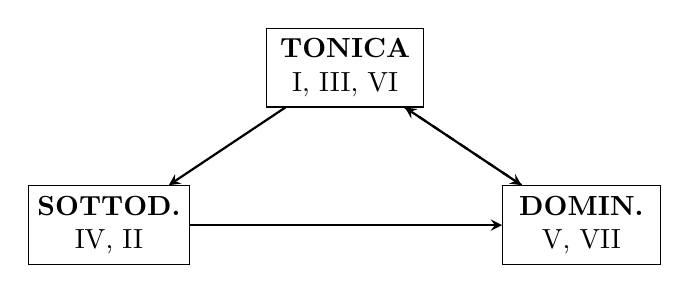
\begin{tikzpicture}[
	box/.style={draw, minimum width=2cm, minimum height=1cm, align=center},
	arrow/.style={->, >=stealth, thick}
]
\node[box, fill=white] (T) at (0,0) {\textbf{TONICA}\\I, III, VI};
\node[box, fill=white] (S) at (-3,-2) {\textbf{SOTTOD.}\\IV, II};
\node[box, fill=white] (D) at (3,-2) {\textbf{DOMIN.}\\V, VII};
\draw[arrow] (T) -- (S);
\draw[arrow] (S) -- (D);
\draw[arrow] (D) -- (T);
\draw[arrow, dashed] (T) -- (D);
\end{tikzpicture}
\end{center}

Il percorso tipico è T $\rightarrow$ S $\rightarrow$ D $\rightarrow$ T, ma è possibile anche il collegamento diretto T $\rightarrow$ D $\rightarrow$ T.
